% \bibliography{../../bibliography/msc_citations}

\section{Student Data}
Events file has 44420509 lines.

\section{Calculation with CouchDB}
As a means of testing feasibility of building indexes across large amounts of documents in CouchDB, I installed the database locally on a Windows 10 personal PC. It took a little over an hour to parse 44 million CSV rows into the database, with nETL using a maximum of around 450MB of system memory and negligible CPU/Disk capacity.

There is no way of calculating indexing times of CouchDB views, so I created a simple index for benchmark purposes:

\begin{minted}{javascript}
function(doc){
    if (doc.type_) {
        emit(doc.type_, 1);
    };
};
\end{minted}

And found that it took a little over 3 hours to build the index on my machine. The view as written above will have to 'touch' every document in the database, allowing a comparative qualitative estimate for the amount of time other indexes will be built. In other words, since an index is already touching every document in the database, the time complexity is O(n) in terms of the document scan and this would hold true regardless of the logic of the index creation itself. So indexes that process a similar number of documents would take a similar amount of time to be created with:

\begin{enumerate}
    \item An allowance for how long it would take to do a linear scan of each document for the 'type\_' property (so documents with more properties would increase index-build time)
    \item An allowance for how many steps the 'emit' function call requires; each of which would require linear scans of document objects and other calculations. i.e. longer documents == longer index-build times.
\end{enumerate}

In terms of the actual indexing itself, CouchDB includes in its installation a query engine identified by 'couchjs.exe'. The actual MapReduce implementation within CouchDB is strictly tied to the Erlang core and could not be altered without major changes to the source code. Opinionated implementation of MapReduce within the CouchDB database stack, makes it's use-case limited compared to other systems that have become synonymous with the 'big-data' stack - including Hadoop, Google xxx, Microsoft xxx, Amazon xxx stacks.

CouchDB's MapReduce pipeline works something along the lines of

\begin{verbatim}
Map Functions executed in parallel, with [key, value] output collected by CouchDB's main Erlang process
=> Grouping
=> Reduce (+/- Rereduce)
\end{verbatim}

The limitations of this pipeline are:

\begin{enumerate}
    \item You can only run the pipeline once. Additional grouping after a reduction is not possible
    \item Handling the rereduce argument makes writing custom reduce functions challenging
\end{enumerate}

For the two reasons mentioned above, although MapReduce CAN be used to implement SQL-like joins, CouchDB's implementation can't be. Instead it is necessary to utilize a 3rd party function to convert grouped [key, value, value, value, value, etc] output from MapFunctions (with group=true) into 'joined' documents. This is easily achievable via two mechanisms:

\begin{enumerate}
    \item Using CouchDB 'list' functions
    \item Using a 3rd party tool external to the CouchDB application itself
\end{enumerate}

todo: mentions couch lists enumerator functionality


\section{Sakai Event data}

\begin{figure}[h]
    \centering
    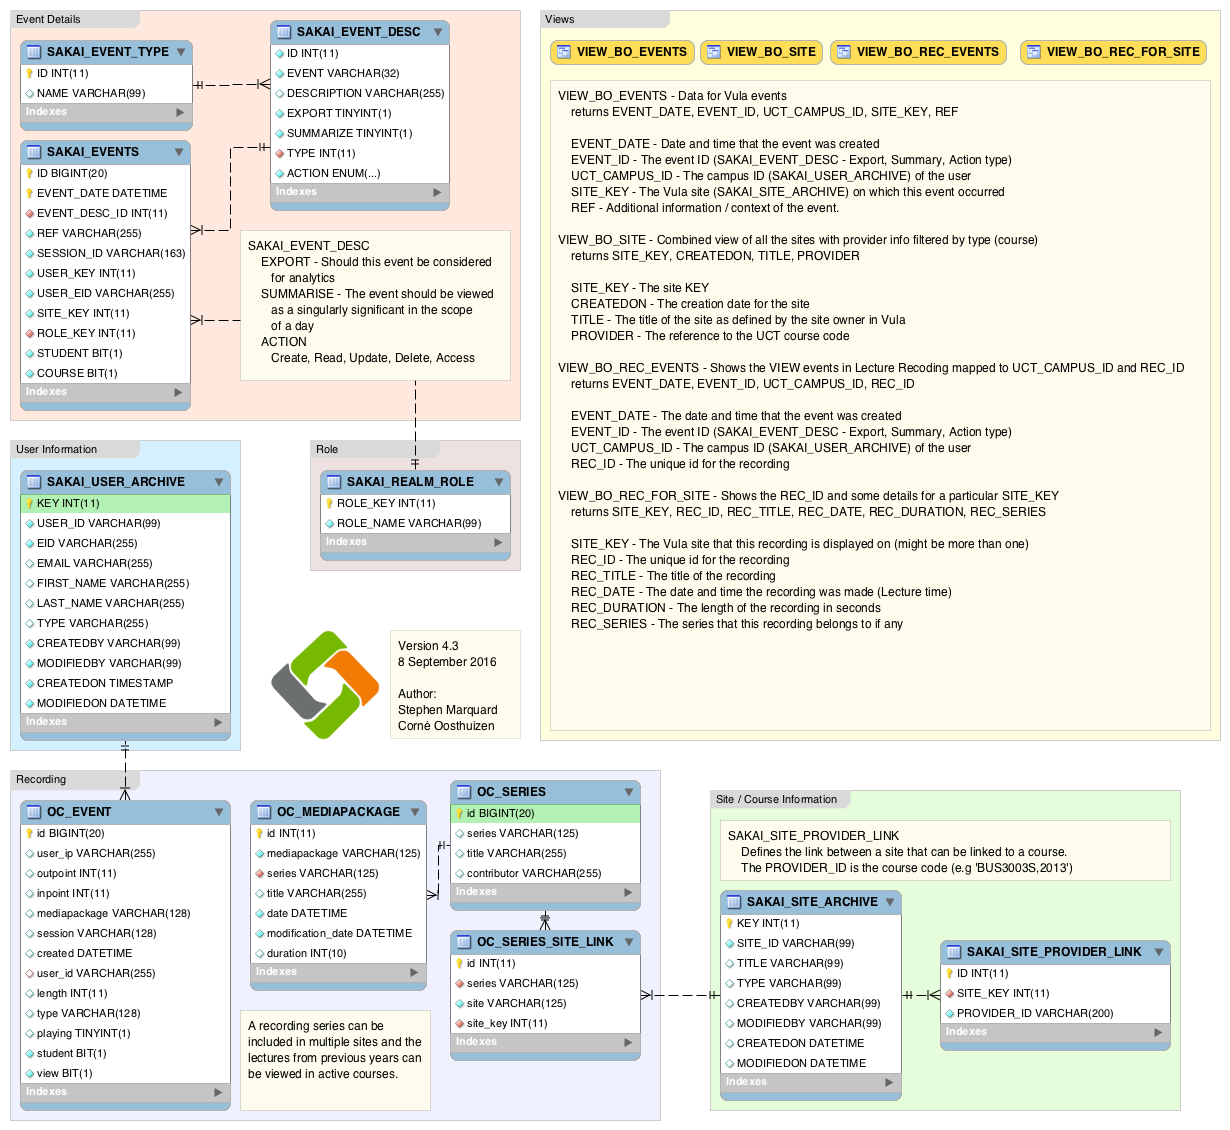
\includegraphics[scale=0.4]{./resources/figures/sakaiEventModel}
    \caption[Sakai]{Model of Sakai browser events as modeled in the RDBMS}
    \label{Sakai}
\end{figure}

Sakai is open source software, meaning that it is fairly straightforward finding information on how it's data-layer is modeled. In this case, browser events are registered as xxx. The University of Cape Town processes the raw event data to model events as represented in \ref{Sakai}. This greatly cuts down on the amount of data that a user needs to process and summarizes all a user's browser interaction on the Sakai site as 'types' of events. These include just 6 categories:

\begin{table}[]
    \centering
    \begin{tabular}{|l|l|}
        \hline
        Event ID & Event Description \\ \hline
        1        & Administration    \\
        2        & Assessment        \\
        3        & Communication     \\
        4        & Content           \\
        5        & Presence          \\
        6        & System            \\ \hline
    \end{tabular}
    \caption[Sakai Event Types]{All user interaction on the Sakai browser frontend can be categorized as a part of one of these events}
    \label{SakaiEventTypes}
\end{table}

\section{3 Way join}

Looking at only events of type 'presence', with reference to the Sakai data model as shown in \ref{Sakai}, it is clear that a natural join (i.e. a join across common columns) is required. Such a join; \textit{R(a,b)} joined with \textit{S(b,c)} joined with \textit{T(c,d)} (where \textit{R}, \textit{S} and \textit{T} are relations and \textit{a}, \textit{b}, \textit{c}, \textit{d} are attributes) could be expressed via the following SQL (SQL Server syntax):

\begin{minted}{sql}
SELECT
[R].[a],
[T].[d]
FROM [R]
LEFT JOIN [S] on [S].[b] = [R].[b]
LEFT JOIN [T] ON [T].[c] = [S].[c]
\end{minted}

As mentioned by \cite{mining2011}, within a MapReduce context such a join can be achieved via:
\begin{enumerate}
    \item A Map function: iterating through all tuples \textit{(commonField, fieldList)} of all relations and producing a key-value pair of the form \textit{(commonField, (Relation, fieldList))}
    \item An implicit group function: group all Map output as a list of tuples per common key of the form \textit{(id, ((R,A), (S, C), (T,D), etc))}
    \item A Reduce function to produce the desirable attributes across the joined tuples \textit{(A,D)} where attribute \textit{C} is of a particular value
\end{enumerate}

As discussed above, a multi-way join is impossible within CouchDB's implementation of MapReduce. As mentioned by \cite{chandar2010} and others xxx multi-way joins need multiple map phases, which is not a possibility using the CouchDB software. CouchDB's implementation of MapReduce is opinionated in that it expects xxx and xxx and doesn't allow for xxx.

TODO: Ask about multiway joins on the Slack channel.